\section{Personas}\label{l:personas}

\begin{table}
\begin{center}
\begin{tabular}{@{}l l}
\textbf{Projektleiter} &\\
\hline
Arthur Blozyk & Sales Information and Communication\\ 
& \trademark{MAN Truck \& Bus AG}\\
Sebastian Nell & Director of USE // Connected Products\\
& \trademark{Scholz \& Volkmer GmbH}\\
Tobias Rudolphi	& Lead Software Architect\\
& \trademark{Zühlke Engineering GmbH}\\
\textbf{Konzept, Design} &\\
\hline
Carsten Fischer	& UX Designer \& Informationsarchitekt\\
& \trademark{triplesense GmbH}\\
Eva Kümml & Senior Konzept / User Experience\\
& \trademark{SinnerSchrader Deutschland GmbH}\\
Sandra-Charlotte Hildebrandt & Dipl. Designerin\\
& \trademark{selbständig}\\
\textbf{Produktion} &\\
\hline
Sebastian Beyer	& Developer\\
& \trademark{Scholz \& Volkmer GmbH}\\
Jan Lochner	& Dipl. Multimedia Producer\\
& \trademark{selbständig}\\
\textbf{Texter} &\\
\hline
Marc Stenzel & Freier Projektleiter, Fachjournalist\\
& \trademark{selbständig}\\
Torsten Schölzel & Freier Texter und Konzeptioner\\
& \trademark{selbständig}\\
\textbf{Übersetzer} &\\
\hline
Jorinde Gessner	& Information Manager\\
& \trademark{Ogilvy \& Mather Deutschland GmbH}\\
\textbf{Kunde} &\\
\hline
Markus Rüb & Sales Information and Communication\\
& \trademark{MAN Truck \& Bus AG}
\end{tabular}
\caption{Interviewte Personen}
\label{table:interviewpartner}
\end{center}
\end{table}

Im vorigen Abschnitt wurden die Probleme geschildert, die im aktuell üblichen Projektverlauf auftreten und daraus gefolgert, was die wichtigsten Aspekte sind, die eine mögliche Lösung behandeln muss. Um den Entwurf eines Systems, dass den verschiedenen Anforderungen entspricht, im nächsten Abschnitt vorzubereiten werden in diesem Abschnitt Personas vorgestellt, die die typischen Benutzergruppen des Systems repräsentieren, und ihre Aufgaben und Erwartungen zusammenfassen. Personas sind ein wichtiger Baustein für den Entwurf eines Systems. Sie ermögliche es, Konzepte und Ideen schon während des Entwurfs zu verfizieren in dem deren Auswirkungen mit dem Nutzungsverhalten und den Erwartungen der Personas verglichen werden.

\begin{quote}
\typoquotes{\textit{Personas describe a site’s target users, giving a clear picture of how they’re likely to use the system, and what they’ll expect from it, among other
things. […] Without personas, there is no common language for talking about what users want.}} \cite[S.15 ff.]{brown2007communicating}
\end{quote}

Personas bilden nicht nur im Entwurf eine wichtige Entscheidungshilfe sondern werden auch während der Umsetzung immer wieder zu Rate gezogen, in dem neue Funktionalitäten auf deren Relevanz und mögliche Probleme für bestimmte Personas hin überprüft werden. \cite[S.38 ff.]{cohn2004user}

\subsection{Überblick}

\begin{figure}[htb]
\begin{center}
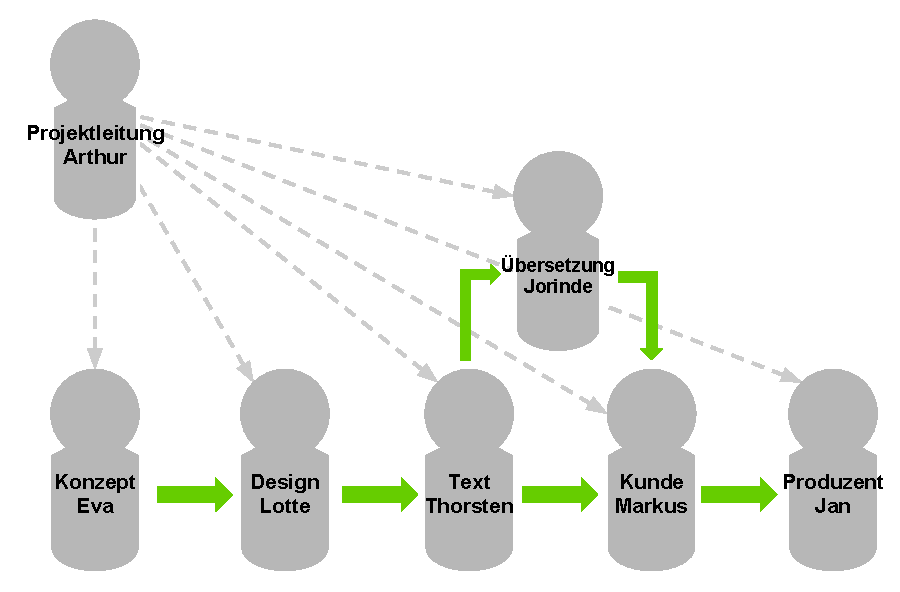
\includegraphics[width=\textwidth]{media/Uebersicht-Personas.pdf}
\caption{Übersicht über die Personas und den idealisierten Workflow}
\label{chart:uebersicht-personas}
\end{center}
\end{figure}

Die nachfolgend vorgestellten Personas basieren auf den im April 2012 geführten Interviews mit den in Tabelle~\ref{table:interviewpartner}~(S.\pageref{table:interviewpartner}) aufgezählten Personen. Die Namen und Fotos der Personas basieren zwar auf den interviewten Personen, dienen aber lediglich dazu, das Merken der Personas zu erleichtern. Die Auswahl der Personas orientierte sich an dem vorherrschenden Workflow innerhalb der Projekte. Wie in Abschnitt~\ref{l:problemanalyse} gezeigt wurde, gibt es in der Praxis keinen linearen Ablauf, sondern es ergeben sich vielzählige Feedback-Schleifen. Beseitigt man aber diese Feedback- und Korrektur-Schleifen kann man die beteiligten Personen in eine, in Abbildung~\ref{chart:uebersicht-personas}~(S.\pageref{chart:uebersicht-personas}) gezeigte, lineare Reihenfolge bringen:
\begin{samepage}\begin{enumerate}\itemsep -5pt
\item Die Konzepterin \emph{Eva}~(\ref{p:eva}) entwickelt das Produkt, wobei sie die Rahmenbedingungen wie Aufbau, Umfang, Zielgruppe, Ansprache festlegt. 
\item Die Designerin \emph{Lotte}~(\ref{p:lotte}) gestaltet das Produkt, wobei sie bestimmt, wie Texte dargestellt werden (Satz, Länge, Schriftart, Farben, Hervorhebungen)
\item Der Texter \emph{Torsten}~(\ref{p:torsten}) erstellt die Texte für das Produkt in der Ausgangssprache
\item Der Kunde \emph{Markus}~(\ref{p:markus}) nimmt die Texte ab
\item Die Übersetzerin \emph{Jorinde}~(\ref{p:jorinde}) übersetzt die Texte
\item Der Produzent \emph{Jan}~(\ref{p:jan}) übernimmt die Texte in das Produkt
\end{enumerate}\end{samepage}

Eine wichtige Rolle fehlt in dieser Aufliste: der Projektleiter \emph{Arthur} koordiniert den Ablauf des Projektes, hat aber keinen Einfluss den Text. Er darf jedoch als wichtiges Bindeglied zwischen allen Beteiligten  nicht fehlen.

Bei der Formulierung der Personas wurde bewusst darauf verzichtet, persönliche Daten wie Alter und Bildung zu verwenden, da diese keinen Einfluss auf den Entwurf des Systems haben. Die Personas enthalten dementsprechend nur 
\begin{itemize}\itemsep -5pt
\item den wichtigsten Nutzen aus der Sicht der Person als Zitat
\item eine Beschreibung der Aufgabe der Rolle, die diese Persona repräsentiert
\item Angaben zu den Beteiligten, mit denen sich die Person im Verlauf des Projektes \emph{über Texte} austauschen wird, Abbildung~\ref{chart:personas-gewichtet}~(S.\pageref{chart:personas-gewichtet}) zeigt diese Beziehungen in einem, nach Anzahl der Kommunikationspartner gewichteten Graphen
\item die verwendeten Werkzeug zur Erfüllung der Aufgabe und die technische Erfahrung
\item die wichtigsten Szenarios, die die Persona mit Hilfe des Systems durchführen wird
\item allgemeine Anforderungen an das System
\item und Angaben darüber, wie der Zugriff auf das System erfolgt.
\end{itemize}

Nachfolgend finden sich die Steckbriefe der einzelnen Personas. 

\pagebreak

\subsection{\emph{Eva}, Konzepterin}\label{p:eva}

\begin{multicols}{2}

\begin{center}
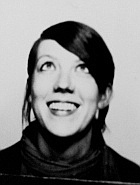
\includegraphics[width=0.5\columnwidth]{media/eva.jpg}
\end{center}

\typoquotes{\textit{Ich möchte, dass alle Beteiligten einen guten Überblick über das Produkt haben.}}

Eva konzipiert als Informationsarchitektin das Produkt. Dabei legt sie entsprechend der Zielsetzung fest, wie das Produkt aufgebaut ist um die Erwartungen des Nutzers zu erfüllen und ihn das gewünschten Ergebnis im Sinne des Produktes leicht erreichen zu lassen. Hierzu erstellt sie einen Überblick über das Produkt mit Hilfe von Wireframes und macht dabei Vorgaben über die Platzierung von Texten und deren Funktion.

\textbf{Organisation, Abstimmung}

Eva arbeitet auf Seite der Agentur und stimmt sich mit \emph{Markus}~(\ref{p:markus}) und \emph{Lotte}~(\ref{p:lotte}) über das Produkt ab. Sie gibt Feedback zu den Texten von \emph{Torsten}~(\ref{p:torsten}) und deren Integration in das Produkt durch \emph{Jan}~(\ref{p:jan}).

\textbf{Werkzeuge und technische Erfahrung}

Evas wichtigstes Werkzeug ist \trademark{OmniGraffle} von \trademark{Omni Group} mit dem sie die Wireframes des Produktes erstellt. Sie ist versiert im Umgang mit vielfältigen Anwendung und steht neuen Werkzeugen offen gegenüber.

\columnbreak

\textbf{Szenarios}

Eva legt fest, welche Text im Produkt verwendet werden. Hierzu definiert sie die einzelnen logischen Bestandteile des Produktes (z.B. Seiten, Abschnitte) und definiert dort die einzelnen Textbausteine.

Eva legt Rahmenbedingungen für den Text fest. Zum einen bestimmt sie die Ansprache, d.h. welche Zielgruppe soll mit den Texten angesprochen werden und welches Ziel verfolgen die Nutzer. Zum anderen macht sie Vorgaben über den Aufbau einzelner Klassen von Texten wie z.B. Überschriften, Schaltflächen, Fließtext bei denen sie z.B. die Textlänge, Spaltenbreite oder Zeilenanzahl festlegt. Diese Rahmenbedingungen kann sie zu den jeweiligen Textbausteinen hinterlegen.

Eva kann sich eine Übersicht ausdrucken, die alle Bestandteile des Produktes enthält. So kann sie leicht den Überblick behalten.

\textbf{Anforderungen}

Da Eva viel Zeit mit der Definition des Produktes, der Texte und der Rahmenbedingungen verbringt, müssen diese Funktionen einfach zu bedienen sein. Sie will nie die Übersicht verlieren und leicht Elemente verändern können, da sich in der Konzeptionsphase häufig Änderungen ergeben. 

Eva hat hohe Ansprüche an die Usability und die Gestaltung des Systems.

\textbf{Zugang}

Eva greift auf das System mit ihrem Laptop zu, sie verfügt über einen großen Bildschirm und eine schnelle Internetverbindung.

\end{multicols}

\pagebreak

\subsection{\emph{Lotte}, Designerin}\label{p:lotte}

\begin{multicols}{2}

\begin{center}
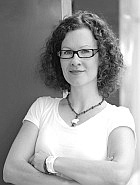
\includegraphics[width=0.5\columnwidth]{media/lotte.jpg}
\end{center}

\typoquotes{\textit{Ich möchte, dass meine Vorgaben zur Gestaltung der Texte von allen berücksichtigt werden.}}

Lotte gestaltet als Art-Direktorin das Produkt. Sie entwirft dazu das Fein-Layout auf Basis der Wireframes, die von Eva~(\ref{p:eva}) erstellt wurden, indem sie für alle Darstellungs-Varianten präzise Entwürfe anfertigt. Hierbei legt sie auch genaue Vorgaben für die Formatierung der Texte im Produkt fest.

\textbf{Organisation, Abstimmung}

Lotte arbeitet auf Seite der Agentur und stimmt sich mit \emph{Eva}~(\ref{p:eva}) bei der Gestaltung des Produktes ab. Mit \emph{Torsten}~(\ref{p:torsten}) spricht sie über ihre Vorgaben zu Texten und überprüft deren Einhaltung in der Umsetzung durch \emph{Jan}~(\ref{p:jan}).

\textbf{Werkzeuge und technische Erfahrung}

Lotte arbeitet mit den Produkten der \trademark{Adobe Creative Suite}. Sie ist nur im Umgang mit wenigen anderen Werkzeugen versiert steht neuen Anwendungen aber offen gegenüber.

\textbf{Zugang}

Lotte greift auf das System mit ihrem Laptop zu, sie verfügt über einen großen Bildschirm und eine schnelle Internetverbindung.

\columnbreak

\textbf{Szenarios}

Lotte erstellt einen Styleguide und legt dabei fest, welche Text-Klassen im Produkt verwendet werden. Text-Klassen sind z.B. Überschriften, Untertitel und Fließtext. Dazu macht sie für jede Klasse Angaben zu der verwendeten Schriftart, die Einschränkungen, wie z.B. die maximalen Zeilenanzahl oder Menge der Zeichen pro Zeile.

Lotte erstellt Layouts in Form von Screenshots oder Beispielseiten. Hierbei verwendet Sie für die Texte die noch nicht durch \emph{Eva}~(\ref{p:eva}) festgelegt wurden, Blindtexte. Um ein besseres Gefühl für die Inhalte zu bekommen und die Layouts besser mit dem Kunden abstimmen zu können möchte Lotte gerne jetzt schon einige Texte von \emph{Torsten}~(\ref{p:torsten}) in den Layouts verwenden.

Während der Umsetzung des Produktes ergeben sich Änderungen am Styleguide. Sie möchte, dass Jan alle Stellen im Produkt anpasst, die von dieser Änderungen betroffen sind.

\textbf{Anforderungen}

Lotte möchte das Anlegen von Text-Vorgaben unkompliziert und schnell erledigen können. Änderungen müssen jederzeit und ohne großen Aufwand möglich sein. Das System muss leicht verständlich sein, da sie nie viel Zeit damit verbringt. Komplizierte Abläufe würden Sie abschrecken und sie würde statt dessen eine E-Mail schreiben.

Lotte hat sehr hohe Ansprüche an die Gestaltung des Systems.

\end{multicols}

\pagebreak

\subsection{\emph{Torsten}, Texter}\label{p:torsten}

\begin{multicols}{2}

\begin{center}

\includegraphics[width=0.5\columnwidth]{media/torsten.jpg}
\end{center}

\typoquotes{\textit{Zitat}}

\textbf{Organisation, Abstimmung}

\ref{p:eva}
\ref{p:lotte}
\ref{p:jorinde}
\ref{p:markus}

\textbf{Werkzeuge und technische Erfahrung}

\columnbreak

\textbf{Szenarios}

\textbf{Anforderungen}

\textbf{Zugang}

\end{multicols}

\pagebreak

\subsection{\emph{Markus}, Kunde}\label{p:markus}

\begin{multicols}{2}

\begin{center}
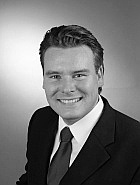
\includegraphics[width=0.5\columnwidth]{media/markus.jpg}
\end{center}

\typoquotes{\textit{Zitat}}

\textbf{Organisation, Abstimmung}

\ref{p:eva}
\ref{p:torsten}
\ref{p:jorinde}

\textbf{Werkzeuge und technische Erfahrung}

\columnbreak

\textbf{Szenarios}

\textbf{Anforderungen}

\textbf{Zugang}

\end{multicols}

\pagebreak

\subsection{\emph{Jorinde}, Übersetzerin}\label{p:jorinde}

\begin{multicols}{2}

\begin{center}

\includegraphics[width=0.5\columnwidth]{media/jorinde.jpg}
\end{center}

\typoquotes{\textit{Zitat}}

\textbf{Organisation, Abstimmung}

\ref{p:torsten}
\ref{p:markus}

\textbf{Werkzeuge und technische Erfahrung}

\columnbreak

\textbf{Szenarios}

\textbf{Anforderungen}

\textbf{Zugang}

\end{multicols}

\pagebreak

\subsection{\emph{Jan}, Produzent}\label{p:jan}

\begin{multicols}{2}

\begin{center}

\includegraphics[width=0.5\columnwidth]{media/jan.jpg}
\end{center}

\typoquotes{\textit{Ich möchte bei Änderungen am Text nicht immer alle Projekt-Dateien anfassen müssen.}}

\textbf{Organisation, Abstimmung}

\ref{p:eva}
\ref{p:lotte}

\textbf{Werkzeuge und technische Erfahrung}

\columnbreak

\textbf{Szenarios}

\textbf{Anforderungen}

\textbf{Zugang}

\end{multicols}

\pagebreak

\subsection{\emph{Arthur}, Projektleiter}\label{p:arthur}

\begin{multicols}{2}

\begin{center}

\includegraphics[width=0.5\columnwidth]{media/arthur.jpg}
\end{center}

\typoquotes{\textit{Zitat}}

\textbf{Organisation, Abstimmung}

Arthur stimmt sich als Projektleiter mit allen Beteiligten ab, hat jedoch keinen Einfluss auf die eigentlichen Texte.

\textbf{Werkzeuge und technische Erfahrung}

\columnbreak

\textbf{Szenarios}

\textbf{Anforderungen}

\textbf{Zugang}

\end{multicols}

\pagebreak

\begin{figure}[htb]
\begin{center}
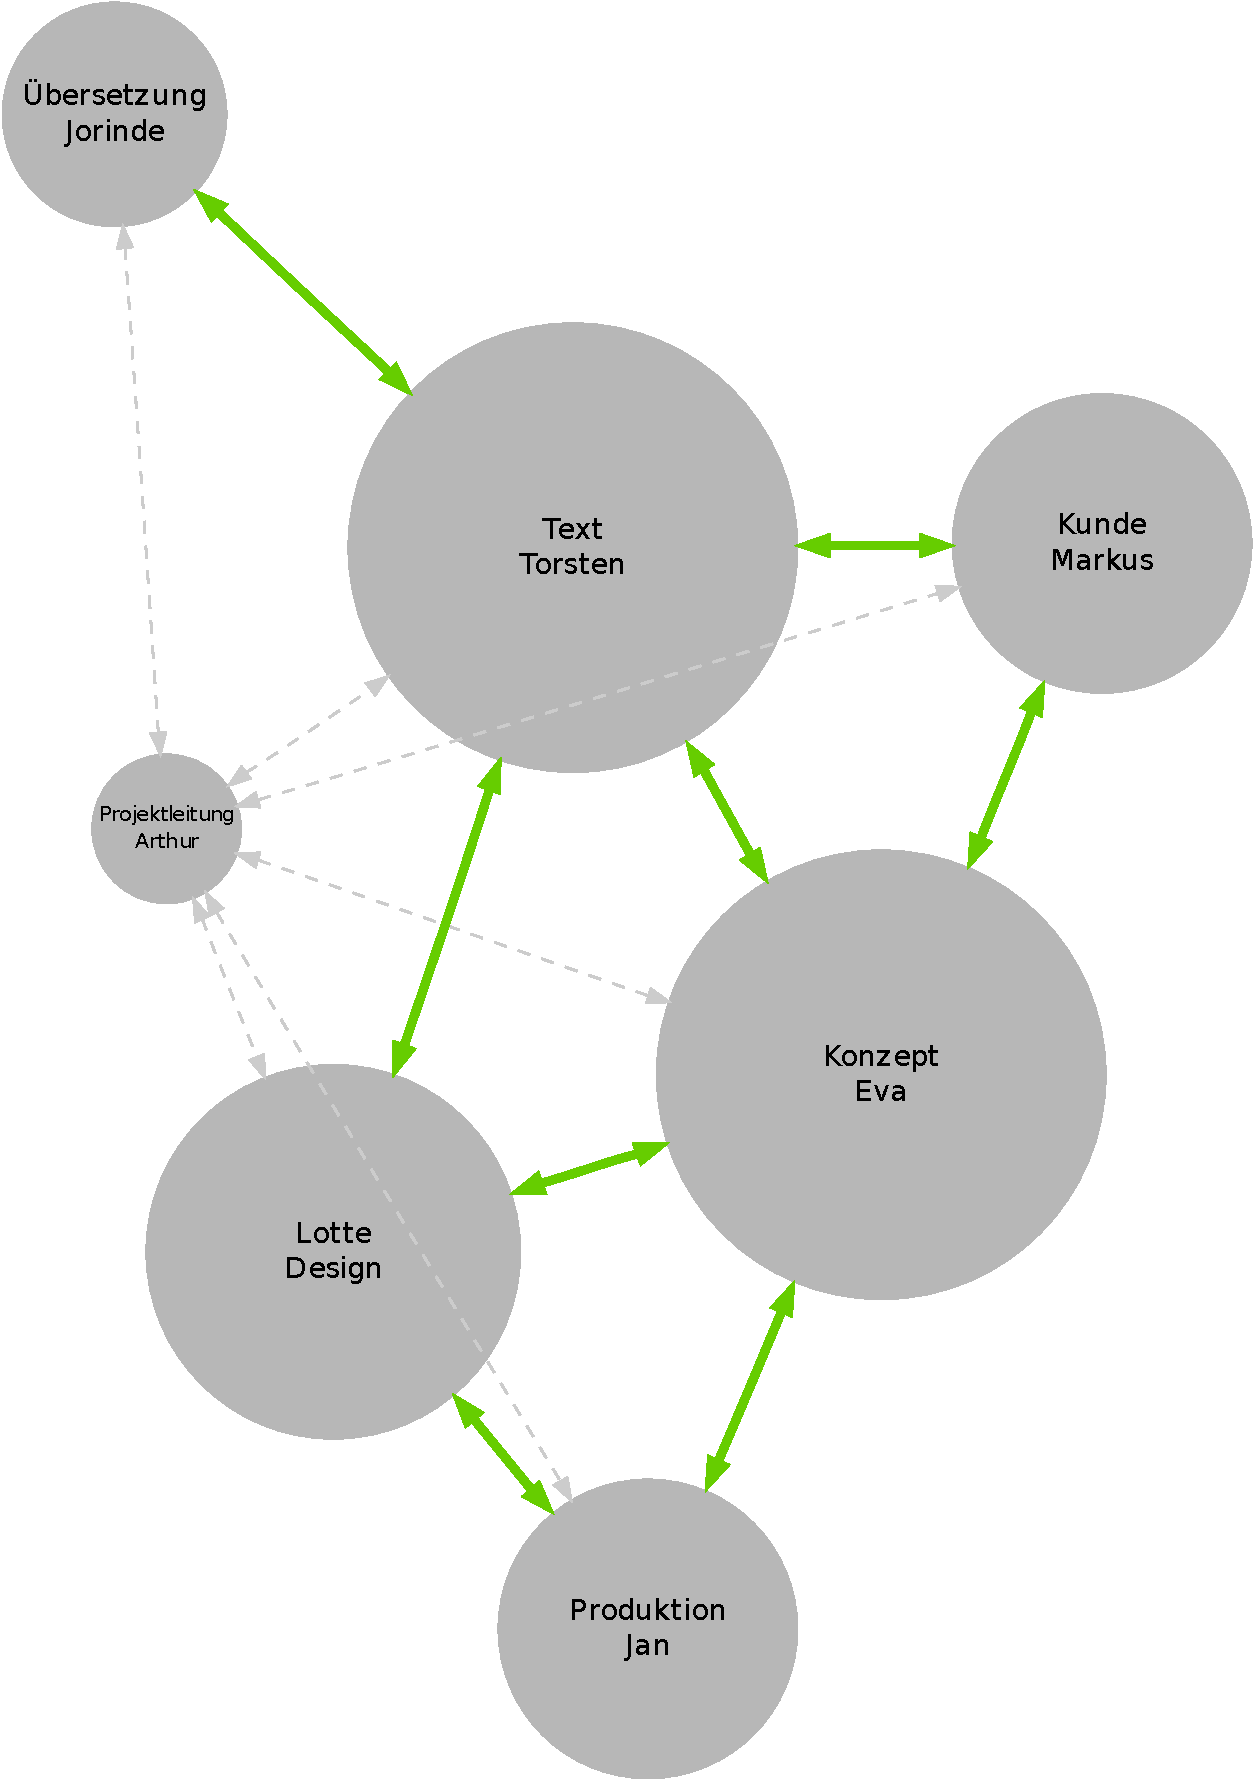
\includegraphics[width=0.55\textwidth]{media/personas-gewichtet.pdf}
\caption{Abstimmung zwischen den Personas, gewichtet nach Anzahl der Kommunikationspartner}
\label{chart:personas-gewichtet}
\end{center}
\end{figure}